\documentclass[10pt,conference,onecolumn,compsoc]{IEEEtran}

\usepackage{hyperref}
\usepackage{enumitem}

\setlist[itemize]{leftmargin=3 cm}
\setlist[enumerate]{leftmargin=3cm}



% *** CITATION PACKAGES ***
%
\ifCLASSOPTIONcompsoc
  \usepackage[nocompress]{cite}
\else
  \usepackage{cite}
\fi



% *** GRAPHICS RELATED PACKAGES ***
%
\ifCLASSINFOpdf
   \usepackage[pdftex]{graphicx}
\else
\fi


% correct bad hyphenation here
\hyphenation{op-tical net-works semi-conduc-tor}


\begin{document}
%title
\title{Financial Database Manager}

%author names
\author{Cody Gonsowski}% <-this % stops a space

% As a general rule, do not put math, special symbols or citations
% in the abstract or keywords.
\IEEEtitleabstractindextext{%
\begin{abstract}
This financial database manager is meant to help users keep track of their finances. It can display expense and income information over an extended timeframe and allows the user to navigate to a range of days' information through a user interface. The target audience is anyone seeking to have more financial stability, but people can easily use it for casual financial tracking. Timeline and the baseline project were most recently completed.
\end{abstract}
}


% make the title area
\maketitle


\IEEEdisplaynontitleabstractindextext
\IEEEpeerreviewmaketitle


\section{Introduction}
This is a financial database manager that allows users to track expenses and incomes over time. Most young adults, especially college students, have a hard time with money, either from a lack of funds or from spending irresponsibly. If bad financial habits go unchecked, a person can potentially get trapped in a vicious cycle of day-to-day living and high outgoing payments. Even if people are not having a hard time with money, it still helps to develop good habits for the future as soon as possible.

The goal is to provide users with a database manager that allows for them to easily view how much they are making or spending over a given period of time. By allowing users to enter (any number of) financial data entries, they will be able to easily see their spending habits over a range of time. The program also provides a total for the range.


\subsection{Background}
The primary goal of this project is to keep a localized database of incomes and expenses that are entered by the user. This allows for the user to easily view any number of entries in a given range. Users will be able to see detailed descriptions of financial data they provide, given they input a sufficient description.

I believe that not only will this project will be challenging but also it will provide something practical. Suppose a person uses a paperback financial planner to keep track of funds. S/he would like to have an online planner to use in their day-to-day life to manage their own finances, but that seems a bit out of reach at this point. In this way, it came to be a locally usable program for database management.


\subsection{Challenges}
Because the program seemed relatively straightforward, I was unsure of all the challenges to come. However, challenges I expected to come across included as follows: on-demand creation of database entries and financial display that shows all entries in a given range.

The on-demand creation of database entries was relatively straightforward. Once I understood how to use OleDB stuff better, it became very easy.
Financial display was handled via a FlowDocument + a Table. This was to show an organized representation of the data that is uniformly formatted.

%As you overcome these challenges, this section becomes more of a retrospective: don't only identify the challenge, but also briefly outline the solution!

%HEREEEEEEEEEEEEEEEEE
\section{Scope}
The user will be able to add an entry to the database through simple form controls. By providing this information, they will be able to add an entry to the database through a simple click. The user will also be able to select a range of dates and display it as a formatted table on a large portion of the application window. The range of dates can vary greatly, and the table should be able to support it through a scroll bar. A total row will be displayed at the bottom of the table that shows the total of the given range.

Some stretch goals we would like to implement to provide a fuller user experience include as follows: clickable calendar interface and a graphical representation of the data.

\subsection{Requirements}
Users can keep the database stored locally so their own form(s) of security will help cover it. Ensuring that the database scales well with large amounts of information allows for users to input data freely.

\subsubsection{Functional}
\begin{itemize}
\item User needs to have a local financial database
\item User can edit the database directly, and the database should be changed when running the manager
\item Calendar date selection should be locked to only valid, calendar-standard inputs
\end{itemize}

\subsubsection{Non-Functional}
\begin{itemize}
\item Operability -- interface should be easy to understand and use
\item Scalability -- database should be able to handle many years' worth of information
\end{itemize}

\subsection{Use Cases}
%This subsection is arguably part of how you define your project scope (why it is in the Scope section...).  In a traditional Waterfall approach, as part of your requirements gathering phase (what does the product actually \emph{need} to do?), you will typically sit down with a user to develop use cases.

%You should have a table listing all use cases discussed in the document, the ID is just the order it is listed in, the name should be indicative of what should happen, the primary actor is typically most important in an application where you may have different levels of users (think admin vs normal user), complexity is a best-guess on your part as to how hard it should be.  A lower number in priority indicates that it needs to happen sooner rather than later.  A sample table, or Use Case Index can be seen in Table \ref{tab:useCaseIndex}.

%use case table
\begin{table}
\centering
\begin{tabular}{|c|c|c|c|c|}
\hline
Use Case ID & Use Case Name & Primary Actor & Complexity & Priority \\
\hline \hline
1 & Date range & User & Med & 1\\
\hline
2 & Add entry & User & High & 2\\
\hline

\end{tabular}
\caption{Use case table}
\label{tab:useCaseIndex}
\end{table}

%use case 1
\begin{itemize}
\item[Use Case Number:] 1
\item[Use Case Name:] Date range
\item[Description:] User selects range of dates they wish to view. They will click on the "Display" button. This will update the table accordingly.
\end{itemize}

\begin{enumerate}
\item User enters the initial date of the range
\item User enters the final date of the range
\item User clicks "Display"
\item Financials table will display information of dates in the range
\item[Termination Outcome:] The Financials table is updated to display the information in the given range.
\end{enumerate}

%use case 1, alternative 1
Alternative: Input is null
\begin{enumerate}
\item User clicks "Display" without anything in start or end date
\item Error will appear indicating no start date
\item If there was a start date, then an error will appear indicating no end date
\item[Termination Outcome:] The user's planner display is left unchanged.
\end{enumerate}

%use case 2
\begin{itemize}
\item[Use Case Number:] 2
\item[Use Case Name:] Add entry
\item[Description:] A user would like to add an entry to the database. They will fill out the three fields (amount, date, and description) and click the "Add" button. This will add the entry to the database.
\end{itemize}

\begin{enumerate}
\item User selects an entry date using the date picker
\item User enters an amount
\item User enters a description (or doesn't)
\item User clicks on the "Add" button
\item Entry will be stored in the database
\item[Termination Outcome:] The database will now contain another entry made by the user. (NOTE: does not dynamically update Financials table if entry is in range)
\end{enumerate}

%\begin{figure}[ht!]
%\includegraphics[height=250px, width=350px]{cat1.jpg}
%\caption{First picture, this is a kitten, not a use case diagram}
%\label{cat1}
%\end{figure}

\subsection{Interface Mockups}
Three objects that allow the user to input, DecimalUpDown (restricts to numerical values), DatePicker (calendar selection of date), and Description (textbox entry)
 "Add" Button allows user to add this in one click.
Date range selection utilizes two DatePickers for easy selection.
"Display" Button allows user to update Financials table in one click.

\begin{figure}[ht!]
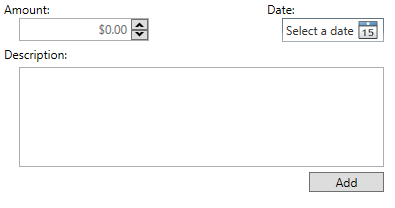
\includegraphics[scale=1]{AddEntry.png}
\caption{By filling out the form and clicking "Add," the user can add an entry to the database.}
\label{AddEntry}
\end{figure}

\begin{figure}[ht!]
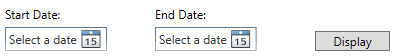
\includegraphics[scale=1]{DateRange.png}
\caption{By selecting a Start and End Date, the user can click "Display" to display the information in \ref{FinancialsTable}.}
\label{DateRange}
\end{figure}

\begin{figure}[ht!]
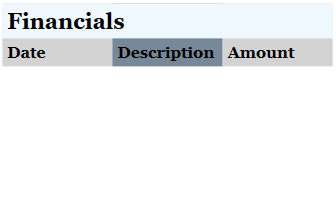
\includegraphics[scale=1]{FinancialsTable.png}
\caption{Display information from \ref{DateRange} will appear here.}
\label{FinancialsTable}
\end{figure}

\section{Project Timeline}
Timeline vaguely looks like... See Figure \ref{Timeline}. Majority of the project's lifetime was spent doing prep work through UMLs and filling out documentation. Majority of the actual programming took place towards the end.

\begin{figure}[ht!]
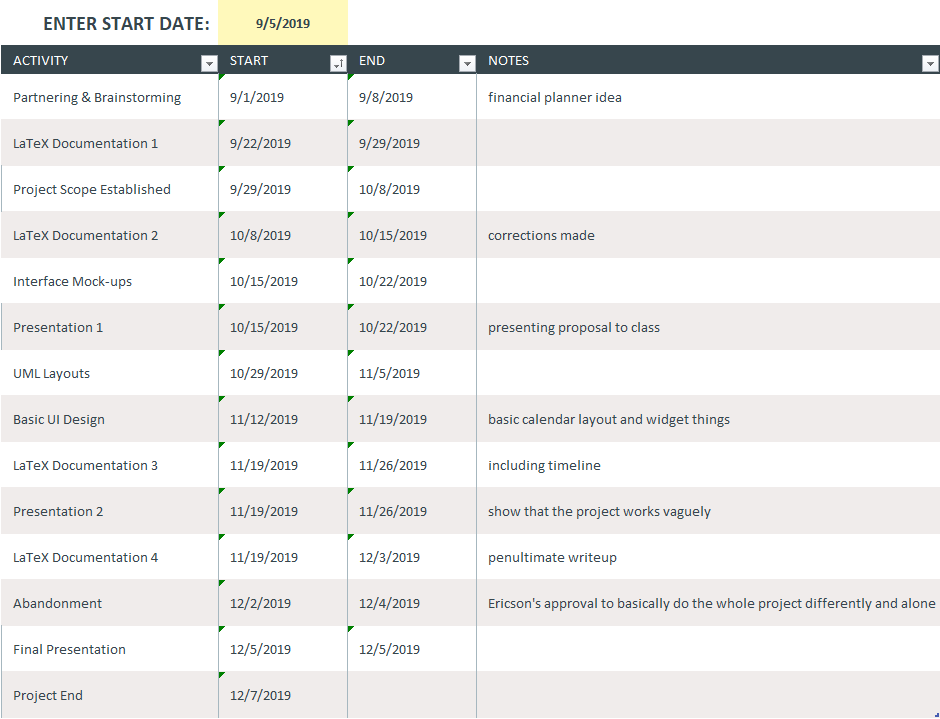
\includegraphics[height=350px, width=500px]{Timeline.png}
\caption{This is a timeline!}
\label{Timeline}
\end{figure}

\section{Project Structure}
MainWindow utilizes DisplayDataRange and AddEntry to provide easy-to-use interfaces for the user.

\subsection{UML Outline}
UML vaguely looks like... See Figure \ref{UML}. MainWindow utilizes two main functions: DisplayDataRange and AddEntry. DisplayDataRange takes the StartDatePicker's and EndDatePicker's entered dates to determine what should be displayed in the table. AddEntry takes the Amount, Date, and Description entered into the form to create a new entry in the database that can be loaded up later.

\begin{figure}[ht!]
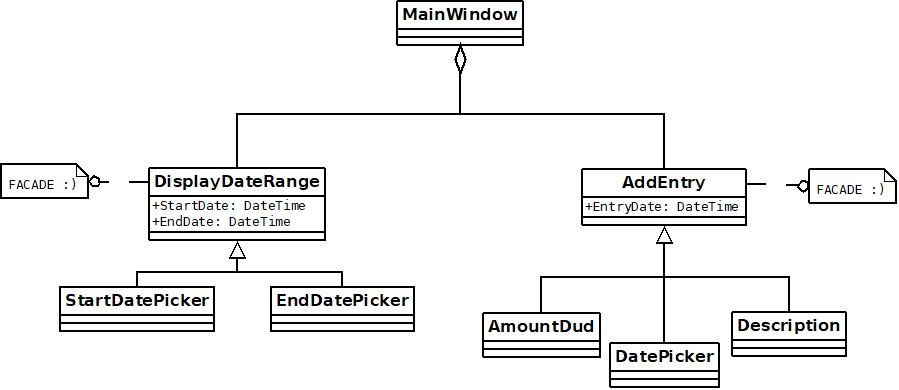
\includegraphics[height=200px, width=500px]{FinancialDMDiagram.jpg}
\caption{Poorly put together UML layout. Did not utilize classes as well as I should have.}
\label{UML}
\end{figure}

%\begin{figure}[ht!]
%\includegraphics[scale=1.5]{cat2.jpg}
%\caption{Your figures should be in the \emph{figure} environment, and have captions.  Should also be of diagrams pertaining to your project, not random internet kittens}
%\label{cat2}
%\end{figure}

\subsection{Design Patterns Used}
AddEntry provides an easy to use interface (Facade) for the user to add new entries to the database, without the user having to go enter everything directly into the database: The program takes care of this.
DisplayDateRange also allows the user to select two dates and display that range of dates, without the user having to sift through all of the database entries manually.

\section{Results}
Unfortunately, many of the project's original goals were not accomplished. The original interface needed a rework to account for change of plans, but hopefully this can be changed in the future to fit a calendar-based interface as originally planned. Some new challenges arose along the way as well, such as working with interworking GUIs, that I was unable to conquer within the timeframe. This should be something to overcome later when implementing the calendar-based interface.

\subsection{Future Work}
It would be ideal to have the planner further developed with a calendar-based interface. This would be easier to see all finances at a glance.
Allowing multiple users to use the same build of the program through user accounts would be beneficial.
On that same note, going online with the database storage would allow people with the build to access their personal database from anywhere.

% that's all folks
\end{document}


